\section{Results}

In this section, we highlight five tile sets that represent different aspects of the
benefits and pitfalls of the Punch Out Model Synthesis (POMS) algorithm.

We start with a brief review of the automatic tile constraint creation.
Though automatic tile constraint creation is a distinct topic from Constraint Based
Tile Generation (CBTG), the two are closely related as any CBTG algorithm requires
a tile constraint set to run.

\begin{figure*}[ht]
  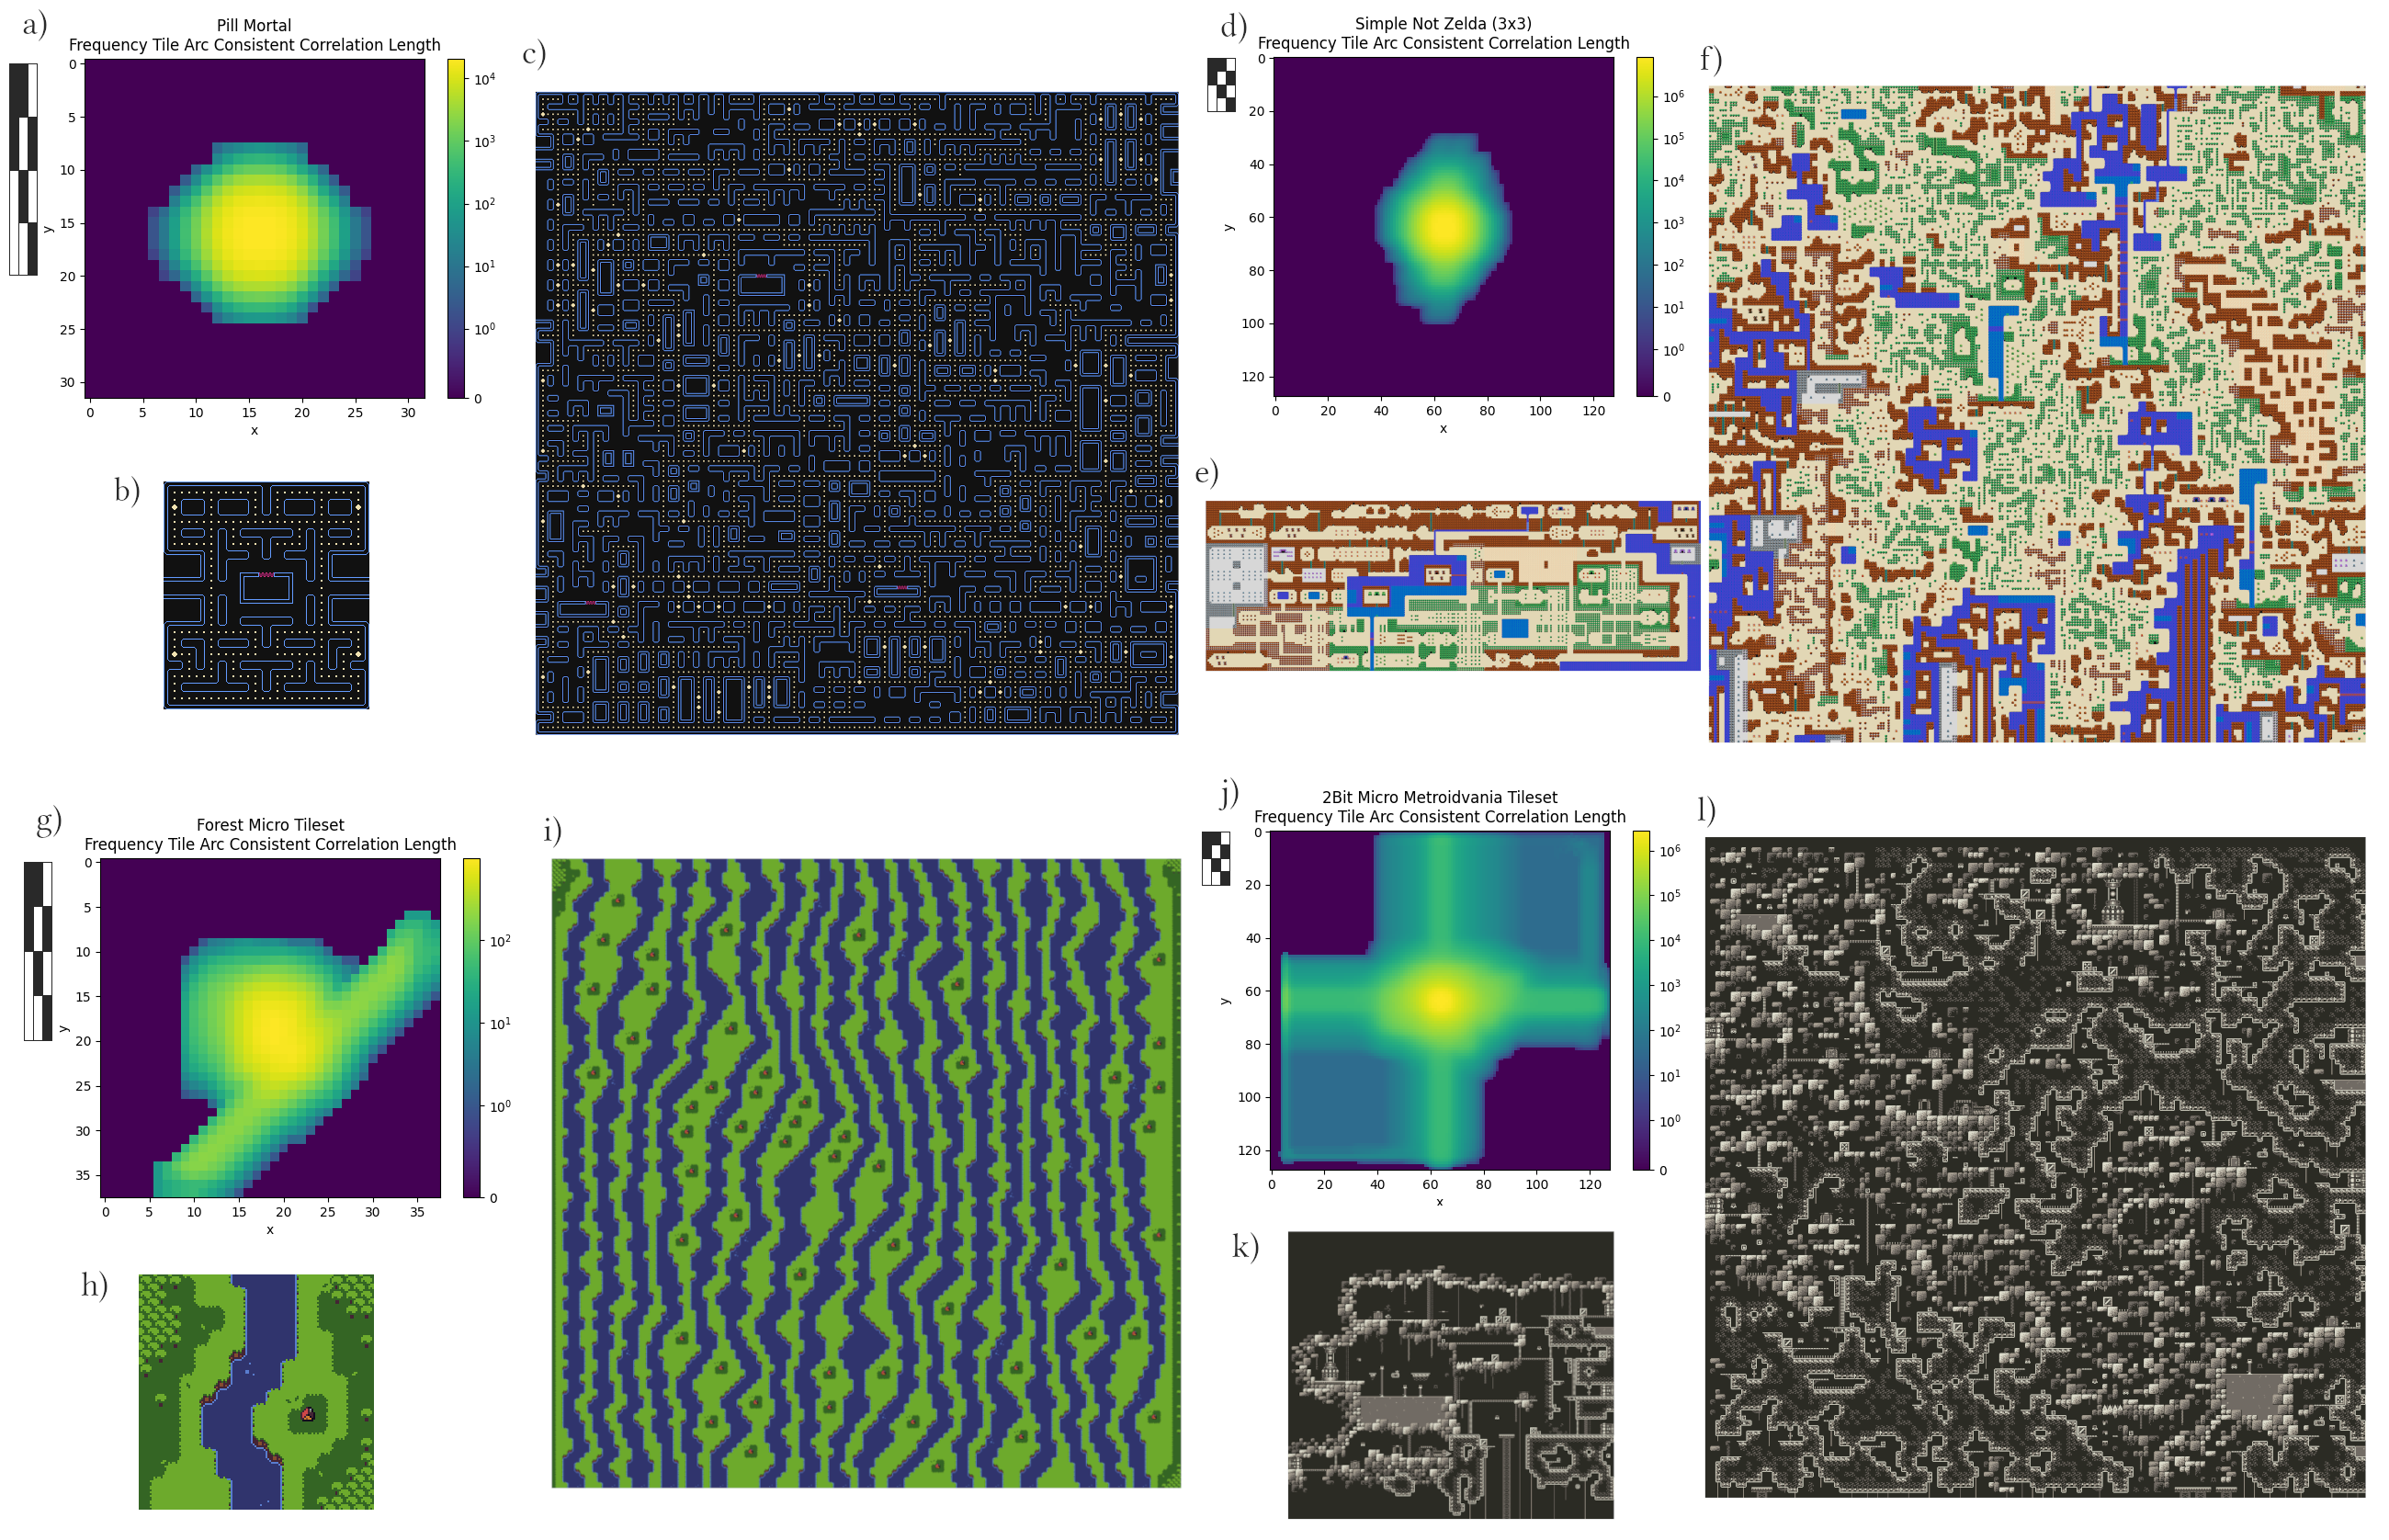
\includegraphics[width=\textwidth]{2d_poms_examples.png}
  \caption{Tile Arc Consistent Correlation Length (TACCL) plots, source exemplar image and example output for four 2D tile sets as listed in Table \ref{table:tilesets}.
           The TACCL, exemplar image and example 64x64 output using a block size of 8x8 for the \textit{Pill Mortal} tile set are shown in a), b) and c) respectively. The TACCL, exemplar image and an example 256x256 output using a block size of 50x70 for LUNARSIGNALS' \textit{Overhead Action RPG Overworld} are shown in d), e) and f) respectively. The TACCL, exemplar image and an example 128x128 output using a block size of 48x48 for Wo\'zniak's \textit{Forest Micro} tile set are shown in g), h) and i) respectively. The TACCL, exemplar image and an example 128x128 output using a block size of 48x48 for 0x72's \textit{Two Bit Micro Metroidvania} tile set are shown in j), k), l) respectively. }
  \label{fig:2dexamples}
\end{figure*}

\begin{figure}[h]
  \centering
  \includegraphics[width=\linewidth]{brutal-plum_cons.png}
  \caption{The Tile Arc Consistent Correlation Length (TACCL) plot, source tile set and an example 32x32x32 output for the 3d \textit{Brutal Plum} tile set listed in a), b) and c) respectively. A block size of 22x22x22 was used.}
  \label{fig:brutal_plum}
\end{figure}

\subsection{Automatic Tile Constraint Creation}

\begin{figure}[h]
  \includegraphics[width=\linewidth]{tileset_rrti.png}
  \caption{a) The exemplar image, take from Wo\'zniak's Forest Micro tile set with a single tile highlighted in red with it's neighbors, as they appear in
           the exemplar image highlighted in orange.
           b) The inferred tile set, packed into an image with the highlighted tile in red and its neighbor tiles highlighted in orange. Note that even though
           tiles in the tile set might look the same, these represent different tiles as they have different constraints for which neighbors are permissible.
           c) A catalog of super tiles, with the highlighted tile in red and its neighbors highlighted in orange. Each super tile consists of a 2x2 window
           taken from the exemplar image (a). Neighbors are derived from the corresponding overlap of the 2x1 tile window  for left and right neighbors and
           a 1x2 tile window for the up and down neighbors. Grey regions represent tiles that fall outside of the exemplar image. }
  \label{fig:rrti_tileset}
\end{figure}

The four 2D tile sets had their tile constraints inferred from an exemplar image using
an automated tile constraint generation method.
The exemplar image is split into tiles and a sliding super tile window, of a larger size than the tile itself, is moved over the exemplar image.
The super tiles are deduplicated and checked for overlapping bands to other super tiles.
For every matching, overlapping band, a tile constraint is added, allowing an admissible pairing for the tiles in the
appropriate dimension direction.

Figure \ref{fig:rrti_tileset} shows the exemplar image (\textit{a}), the inferred tile set (\textit{b}) and the complete list of super tiles
for Wo\'zniak's \textit{Forest Micro} tile set (\textit{c}).
A single tile is highlighted in red and its neighbors are highlighted in yellow with red edges corresponding to their neighboring direction.

Figure \ref{fig:rrti_tileset} uses a tile size of 8x8 pixels, with a 2x2 super tile size.
The upper left hand tile is used as the displayed representative tile, which can be seen by comparing the non dimmed tiles in the
super tile list from Figure \ref{fig:rrti_tileset} (\textit{c}) to the packed tile set image (\textit{b}).
A 2x1 overlapping band is in each direction, suitably rotated, to find which super tiles neighbor other super tiles.
An interested reader can confirm that there is a 2x1 overlap to the highlighted red super tile to each of its highlighted yellow neighbors
in Figure \ref{fig:rrti_tileset}.

Boundary constraints need special consideration.
One option is to only allow a special ``zero'' tile at grid boundaries, ensuring ``zero'' tile constraints are added
for tile pairs that fall across the edge boundaries of the exemplar image.
This is the option chosen for Wo\'zniak's \textit{Forest Micro} tile set and can be seen in the ``zero'' (gray) tiles present for
the super tiles listed in Figure \ref{fig:rrti_tileset} (\textit{c}).
Another option is to have \textit{wrap around boundary conditions}, with a sliding window that wraps right or up to left or down directions, respectively,
and is the method chosen when creating the tile constraints for LUNARSIGNALS' \textit{Overhead Action RPG Overworld} tile set.

If the tile constraints include the ``zero'' tile at the grid boundaries, this will be denoted as \textit{hard boundary conditions}.

%The term \textit{wrap around boundary conditions} will be used when the tile constraints are constructed with wrap around boundary conditions.

For the automatic tile constraint creation from exemplar images, some artistic input is needed in choosing tile size, window size and boundary conditions.
The tile sizes, window sizes and boundary conditions for the 2D tile sets used in this paper were chosen through inspection and experimentation.
An in depth explanation of automatic tile constraint creation is beyond the scope of this paper and readers are referred to \cite{Gumin_2016, Sherratt_2019, BorisTheBrave_wfc_2021} for further details.
The five tile sets we use here are summarized in Table \ref{table:tilesets}.

%\subsection{Tile Arc Consistent Correlation Length}
%
%As a simple, measurable quantity to help understand the correlation length implied by the tile constraints, we define a Tile Arc Consistent Correlation
%Length (TACCL), as first mentioned in Hoetzlein's \texttt{just\_math} project \cite{Hoetzlein_2023}.
%The computation of the TACCL is done as a pre-processing step independent of the POMS algorithm.
%The idea is to iterate through each tile in isolation and record the maximum distance constraint propagation reaches when resolving a center cell.
%
%Starting from a small test grid set to an indeterminate state,
%the center cell is resolved to a tile and constraint propagation is performed to put the grid
%into an arc consistent state.
%The size of a bounding box that minimally encompases every cell whose tile domain was altered during the constraint propagation is then saved.
%The grid is then reverted to an indeterminate state and the next tile is chosen to resolve, repeating the process and updating the maximum distances
%of the minimum encompasing bounding box for each tile tested.
%
%The Tile Arc Consistent Correlation (TACCL) is the maximum extent of the saved bounding boxes from iterating through all tiles.
%Algorithm \ref{alg:taccl} provides psuedo-code for the TACCL calculation.
%
%\begin{algorithm}
%  \caption{Tile Arc Consistent Correlation Length}
%  \label{alg:taccl}
%  \begin{algorithmic}
%    \State \textbf{Output:} Tile Arc Consistent Correlation Length $L$
%    \State \textbf{Input:} Block Size $(M _ x, M _ y, M _ z)$
%    \State Create a block $B$ of size $(M _ x, M _ y, M _ z)$
%    \State Put block $B$ in a fully indeterminate state
%    \State $L=1$
%    \For { tile every tile $t \in D$ }
%      \State $B' = B$
%      \State Apply initial setup restrictions to $B'$
%      \State Resolve center cell, $c$, in $B'$ to $t$
%      \State Make $B'$ arc consistent
%      \State Find mininum bounding box, $bbox$, \\ \ \ \ \ \ \ \ \ encompassing altered cells of $B'$
%      \If{ $\max _ { x, y, z } bbox  > L$ }
%        \State $L = \max _ { x, y, z } bbox $
%      \EndIf
%    \EndFor
%    \State Return $L$
%  \end{algorithmic}
%\end{algorithm}
%
%For the sake of brevity, no checks are performed in Algorithm \ref{alg:taccl} to determine if the calculated value
%is as large as the input block size ($M _ x, M _ y, M _ z$).
%In such a case, either the TACCL is unbounded or the test block size is smaller than the TACCL and the test block size would
%need to be increased.
%
%The TACCL is meant to estimate the correlation length of an underlying tile constraint set but can be misleading as some
%tile constraints will have a finite TACCL even though correlation lengths can be unbounded.
%An unbounded TACCL implies an unbounded correlation length but the converse is not true and a finite TACCL
%does not necessarily imply a finite correlation length.
%The \textit{Brutal Plum} tile set, that has an unbounded correlation length but finite TACCL,
%displays this phenomenon and will be discussed later in this section.

%      \specialcell{Window Size \\ (in tiles)}  & $2 \times 2$ & $3 \times 3$ & $2 \times 2$ & $2 \times 2 $ & n/a \\
%      \specialcell{Overlap \\ (in tiles)}  & $1 \times 2$ & $2 \times 3$ & $1 \times 2$ & $1 \times 2 $ & n/a \\
%\def\checkmark{\tikz\fill[scale=0.4](0,.35) -- (.25,0) -- (1,.7) -- (.25,.15) -- cycle;} 
%      \specialcell{Boundary \\ \ \ Conditions} & \textit{H} & \textit{W} & \textit{H} & \textit{H} & \textit{H} \\
%      \cline{1-1} 

\begin{table}[h]
  \centering
  \begin{tabular}[t]{l|ccccc}
    & \textit{PM} & \textit{OARPGO} & \textit{FM} & \textit{2BMMV} & \textit{BP} \\
    \hline
      Dimension & 2D & 2D & 2D & 2D & 3D \\
      Tile Size (px) & 8px & 16px & 16px & 24px & n/a \\

      \textit{SuperTile} & & & & & \\
      \specialcell{\ \ Window }  & 2x2 & 3x3 & 2x2 & 2x2 & n/a \\
      \specialcell{\ \ Overlap }  & 1x2 & 2x3 & 1x2 & 1x2 & n/a \\
      Tile Count & 190 & 3031 & 159 & 1807 & 90 \\
      \hline

      \specialcell{\textit{Boundary} \\ \ \ \textit{Conditions}} & & & & & \\
      Hard & \checkmark & & \checkmark & \checkmark & \checkmark \\
      Wrap & & \checkmark & & & \\
      \hline

      \specialcell{\textit{Block Choice} \\ \ \ \textit{Scheduler}} & & & & & \\
      Uniform & \checkmark &  & & \checkmark & \checkmark \\
      Diagonal & & & \checkmark & & \\
      Center Out & & \checkmark & & & \\

      \hline
      TACCL (x/y) & 24 & 50/70 & $\infty$ & $\infty$ & 16 \\
      Block Size & 32 & 50x70 & 48 & 48 & 22 \\

     \hline
  \end{tabular}
  \caption{\textit{Pill Mortal} (\textbf{PM}) tile set \\ \textit{Overhead Action RPG Overworld} (\textbf{OARPGO}) tile set \cite{LUNARSIGNALS_oarpgo} \\ \textit{Forest Micro} (\textbf{FM}) tile set \cite{ThKaspar_micro} \\ \textit{Two Bit Micro Metroidvania} (\textbf{2BMMV}) tile set \cite{0x72_2bmmv} \\ \textit{Brutal Plum} (\textbf{BP}) tile set}
  \label{table:tilesets}
\end{table}

%  \caption{\textit{Pill Mortal} (\textbf{PM}) tile set \\ \textit{Overhead Action RPG Overworld} (\textbf{OARPGO}) tile set \cite{LUNARSIGNALS_oarpgo} \\ \textit{Forest Micro} (\textbf{FM}) tile set \cite{ThKaspar_micro} \\ \textit{Two Bit Micro Metroidvania} (\textbf{2BMMV}) tile set \cite{0x72_2bmmv} \\ \textit{Brutal Plum} (\textbf{BP}) tile set \\ The \textit{Boundary Condition} denote how the boundaries of the exemplar image are used to create the tile constraints, with the code \textit{H} being ``hard'' boundary conditions with an added ``zero'' tile virtually added around the exemplar image and placed outside of grid boundaries during realization and the \textit{W} code to denote ``wrap around'' boundary conditions\\ The Block Choice Scheduler (\textit{BCS}) strategy has codes \textit{U} for uniform, \textit{C} for ``center out''  and \textit{D} for diagonal}

%The TACCL is an ad-hoc heuristic measure of tile constraint correlation.
%The motivation for the TACCL usage is from an intuition that there are many local energy minima, that are noisy and approximately a correlation length in size, that must
%be overcome in order to make progress.
%A more thorough and detailed analysis typical energy landscapes, correlation length in general and the TACCL in particular is beyond the scope of this paper.

Table \ref{table:tilesets} provides information for five tile sets, \textit{Pill Mortal}, \textit{Overhead Action RPG Overworld},
\textit{Forest Micro}, \textit{Two Bit Micro Metroidvania} and \textit{Brutal Plum}, highlighted in this paper.
The tile size, supertile window and supertile overlap parameter choices are provided as they are used in the automatic tile constraint generation
along with the boundary conditions and the resulting tile count for each tile set.
The Block Choice Scheduler (BCS) and blocks sizes are also provided that were used to generate the example outputs in Figure \ref{fig:2dexamples} and Figure \ref{fig:brutal_plum}.

Here, the \textit{uniform} BCS denotes a block choice schedule that randomely chooses a block centers uniformly from
indeterminate cells in the grid.
A \textit{diagonal} BCS denotes block center choices weighted preferentially to the upper left corner and
\textit{center out} BCS denotes block center choices weighted preferentially towards the center of the grid,
with both restricting choices to indeterminate grid cells.

Figure \ref{fig:2dexamples} and Figure \ref{fig:brutal_plum} show the TACCL, reference images and example runs
for these five tile sets.
We group the 2D tilesets into \textit{bounded} and \textit{unbounded} TACCL, with special consideration for
the \textit{Brutal Plum} tile set.


%The Tile Arc Consistent Correlation length (TACCL), reference images and example runs
%for the tile sets listed in Table \ref{table:tilesets} are shown in 
%Figure \ref{fig:2dexamples} and Figure \ref{fig:brutal_plum}.

%Figure \ref{fig:2dexamples} and Figure \ref{fig:brutal_plum} shows the Tile Arc Consistent Correlation length (TACCL),
%the reference image used to create the tile set and an example run for the four 2D tile sets
%listed in Table \ref{table:tilesets}.

\subsection{Tile Constraints with Bounded TACCL}

The first two tile sets that appear in Figure \ref{fig:2dexamples}, \textit{Pill Mortal} and LUNARSIGNALS' \textit{Overhead Action RPG Overworld}
(OARPGO) tile set,
have bounded Tile Arc Consistent Correlation lengths (TACCL).

The \textit{Pill Mortal} tile constraints were generated from the exemplar image shown (Figure \ref{fig:2dexamples}, label \textit{b}), using
an 8x8px tile size, hard boundary conditions with a 2x2 super tile window, a 1x2 tile overlap and the upper left hand corner tile as the representative
display tile.
The generated realization in Figure \ref{fig:2dexamples} (label \textit{c}) was created from a POMS run with block size 32x32 on a 128x128 grid.
A uniform weighting for all 190 tiles was used.
A uniform block choice scheduler policy was chosen that selected block centers uniformly at random from the set all unresolved grid cells.

LUNARSIGNALS' \textit{OARPGO} tile constraints were generated from the exemplar image shown (Figure \ref{fig:2dexamples}, label \textit{e}), using
an 16x16px tile size, wrap around conditions with a 3x3 super tile window, 2x3 tile overlap and and the middle tile as the representative
display tile.
In this case, a 3x3 window was chosen as a smaller 2x2 window was observed to not give good aesthetic results.

When generating outputs using the OARPGO tile set, the outer frame of the grid is pinned to an unresolved state.
This is necessary as the tile constraint set was created with wrap around conditions and has no valid constraints that match the ``zero'' tile
to the rest of the tile domain.

The example 256x256 output (Figure \ref{fig:2dexamples}, label \textit{f})
was created with a block size of 50x70.
A block choice strategy was used that preferentially chose block centers from unresolved grid cells
nearer to the center.
This has the effect of resolving regions from the \textit{center out}, never creating isolated regions that need to be joined and effectively
  ensuring a large contiguous region during the course of the algorithm.
From observation, other block choice strategies were not as successful as choosing block centers with a grid center bias.

It should be noted that without wrap around boundary conditions, the OARPGO tile set would have unbounded TACCL.
Further, without wrap around boundary conditions POMS has trouble finding solutions as the
grid boundary region is non trivial for this tile set.
The success of the center out block choice strategy, the failure of other block choice strategies and the unbounded TACCL of
non wrap around boundary conditions, could suggest that the bounded TACCL does not capture some longer range or unbounded constraints
  embedded within the wrap around OARPGO tile set constraints.

Of note is the ``stuttering'' effect that happens with many features being repeated in a linear direction.
For example, there are long regions of vertical rocks surrounded by water tiles that continue on downward until the
pinned boundary is hit.
This effect becomes even more pronounced when other tile weightings are used.
We suspect this is because of a certain pattern preference that then gets re-enforced
by a surrounding structure.
We make note of this effect but otherwise don't investigate further in this paper.

\subsection{Tile Constraints with Unbounded TACCL}

The last two tile sets in Figure \ref{fig:2dexamples}, Wo\'zniak's \textit{Forest Micro} tile set and 0x72's \textit{Two Bit Micro Metroidvania} tile set,
both have unbounded Tile Arc Consistent Correlation Lengths (TACCL).

The tile constraints for Wo\'zniak's \textit{Forest Micro} tile set were generated from the exemplar image shown (Figure \ref{fig:2dexamples}, label \textit{h}), using
an 16x16px tile size, hard boundary conditions with a 2x2 super tile window using a 1x2 tile overlap and taking the upper left hand corner tile as the representative
display tile.
The generated realization in Figure \ref{fig:2dexamples} (label \textit{i}) was created from a POMS run with block size 48x48 on a 128x128 grid
and a uniform tile weighting for all 159 tiles.
A diagonal weighted block choice scheduler policy was chosen that selected block centers from the set all unresolved grid cells weighted by their Euclidean distance
to the upper left corner of the grid.

From the local, nearest neighbor pairwise tile constraints,
the \textit{Forest Micro} tile set has an implied global constraint that the river count from the top row of the realized
grid must match the river count on the bottom row.
This global constraint is not explicitly present or specified but is a by-product of the local constraints.

For large grid sizes, POMS fails to find realizations for the \textit{Forest Micro} tile set when a block
choice policy chooses block centers at random.
Under these conditions, POMS effectively makes a random choice for the number of rivers on the top and bottom row.
One can expect, with enough random sampling, the river count to be identical, but the problem
becomes increasingly less likely as grid size grows.

To guide POMS in finding solutions for the \textit{Forest Micro} tile set, a
block choice policy was chosen that preferentially weights cell positions starting from the upper left and decreases as
cells are considered going down and to the right.
The diagonal weighting has the effect of keeping a growing contiguous region that locally keeps the top and bottom
river counts the same.
Contradictions that do occur tend to be localized and their resolution keeps the river counts the same

Though the \textit{Forest Micro} tile set has an unbounded correlation length, the global constraint is weak enough
to be overcome by this simple weighted diagonal heuristic.
%Figure \ref{fig:2dexamples} label \textit{i} shows an example run for a 128x128 grid with a block size of 48x48, using
%the weighted diagonal block choice scheduling strategy heuristic.

The tile constraint set for 0x72's \textit{Two Bit Micro Metroidvania} (2BMMV) tile set was
generated from the exemplar image shown (Figure \ref{fig:2dexamples}, label \textit{k}) with a 24x24 pixel tile size, a 2x2 super tile window
using a 1x2 tile overlap and taking the upper left hand corner tile as the representative display tile.

As can be seen by Figure \ref{fig:2dexamples} (label \textit{j}), the 2BMMV tile set has unbounded correlation length, but the constraint is weak
enough to be overcome by running POMS with a block size of 48x48 and a block choice scheduler that chooses block centers from
unresolved grid cell positions uniformly.
An example output for the 2BMMV for a 128x128 grid using a 48x48 block size and uniform block choice schedule can be seen in \ref{fig:2dexamples} (label \textit{i}).
The unbounded correlation length comes from the boundary restrictions which might disappear if care were taken
to create wrap around tile constraints.

\subsection{Unbounded Correlation Length but Bounded TACCL}

The 3D \textit{Brutal Plum} tile set was programmatically generated from a set of 20 unique tiles that, after rotations and deduplication,
grows to 90 tiles.
Many of the tiles are aesthetically identical but are logically different to embed desired features, such as requiring certain
logical tiles to be above or below other tiles.
In particular, non empty tiles must have a non empty path to the ground base plane, giving an implied global constraint.
The global constraint is not captured by the Tile Arc Consistent Correlation Length (TACCL) and highlights
the failure of the TACCL heuristic to properly capture an unbounded correlation length embedded in the tile set.

Though the correlation length for the \textit{Brutal Plum} tile constraints is unbounded, POMS still is able to reliably find realizations with
block size 22x22x22, an example output of which is highlighted in Figure \ref{fig:brtual_plum} (label \textit{c}).
For aesthetic reasons, a tile weighting that increases the likelihood of the empty tile, the arch tiles and
stair tiles was chosen.
The reader is referred to the reference implementation \footnote{ \label{poms-url} \url{https://github.com/zzyzek/PunchOutModelSynthesis} }
for further details.


